% !TeX root = ../main-english.tex
% !TeX spellcheck = en-US
% !TeX encoding = utf8
% -*- coding:utf-8 mod:LaTeX -*-

%This smart spell only works if no changes have been made to the chapter
%using the options proposed in preambel/chapterheads.tex.
\setchapterpreamble[u]{%
	\dictum[John Claerbout, paraphrased by Buckheit \& Donoho]{An article about computational science in a scientific publication is not the scholarship itself, it is merely advertising of the scholarship. The actual scholarship is the complete software development environment and the complete set of instructions which generated the figures.}
}

\chapter{Introduction}
\label{chap:k1}

Look mom, some text!

\section{Brain state spaces}
This is an introduction into brain states and functional alignment
\pagebreak

\section{Magnetoencephalograpy (MEG)}
This is an introduction into \gls{meg} data

%The signals MEG measures are summed up postsynaptic potentials (IPSP or EPSP, slow-ish ~10ms and monophasic) that primarily originate from synchronized tangential neural activity produced by the parallel pyramidal cells that are perpendicular to the cortical sheet of the gray matter, mostly from the walls of the cortical sulci. The potential differences between soma and axons of neurons form magnetic dipoles, and, when aggregated across a neuronal population, measurable magnetic fields.
%The cortical magnetic fields produced by those signals are tiny, on the order of 10-10³ femtotesla (fT). This is a very weak magnetic field compared to the environmental noise.
%Magnetic flux is a measurement of the total magnetic field which passes through a given area, and is the physical measurement behind MEG.
%While active and passive shielding around the MEG measuring room are used for noise cancellation, flux transformers (input coils), placed as closely to the head as possible, amplify the magnetic field.
%Liquid helium in the dewar around the sensors cools the MEG down to -269°C and makes the flux transformer superconductive. In this state, there can’t be any net current in the flux transformer, and produce a more dense and stronger magnetic field that can be measured with Superconducting Quantum Interference Devices (SQUIDs) which are sensitive detectors of magnetic flux.
%Three main types of flux transformers exist: magnetometer, axial gradiometer, and planar gradiometer. Different flux transformers have a different sensitivity profile.

%Magnetometers are the most simple ones. They have a single coil and measure only one component of the magnetic field. This makes them very sensible to the distance of the source, but also susceptible to environmental noise.

%Gradiometers consist of two magnetometers placed in opposite directions. They exist in planar and axial orientation. Their general advantages are that environmental noise gets cancelled out and that they are as such more sensitive to the magnetic field of the cortical pyramidal sheet. An additional advantage of planar gradiometers is that their sensitivity is largest when placed directly over the dipol (a place where a magnetometer or axial can not pick up signals).
%Regardless of which flux transformer is used, MEG analysis consists of interpreting the resulting topographies given the employed flux transformer. Each flux transformer can be described by its lead field, i.e., how it couples to local source currents, which is very important information in source reconstruction.
%An MEG device can contain different types of flux transformers and the total number of flux transformers is the amount of channels of the MEG system.

%Typically, MEG devices contain around 150-300 sensors (SQUIDs) arranged in a helmet-shaped array that cover the whole human scalp at a frequency of 1000-5000Hz.
%This results in a typical temporal sampling rate of about ~1000Hz, and a typical spatial sampling rate of about ~300 sensors. The spatial topography of the activity is thus harder to pinpoint, but central in MEG analyses to make sense of the aggregated signal from multiple sources from within the brain at the scalp (a problem known as signal superposition - fields produced by several currents are sums of fields generated by each single current).




\pagebreak

\section{Research data management}
%This is an introduction on the importance of research data management for reproducible science

Research data encompasses everything that is produced in the life span of a research project.
From raw data acquisitions, preprocessed or otherwise standardized datasets, to software, analysis scripts, results, compiled reports or articles, figures, and other final or intermediate research outcomes.
To disambiguate the term ``research data'' from the smaller-scoped meaning of ``data'' in colloquial language (the outcome of a data acquisition in an experiment), it is also referred to in the literature as ``research objects``, and, in case it exists in purely electronic form, as ``digital research objects'' \citep{bechhofer2010research}. \\
Typically, research objects have a much longer life span than the project that creates them.
Science is an incremental process that produces and builds up on more than just published journal articles \citep{mons2018data}, and code, data, results, or tools of previous finished or unfinished projects fuel new undertakings.
\gls{rdm} describes the handling of these research objects through their entire life cycle: from curation, use, publication and sharing, archiving to re-use or destruction (\cref{fig:rdm-lifecycle}).
Ultimately, it ensures that research objects are preserved to act as an evidence base for findings, and as a discoverable resource for further reuse.
As I will lay out in this section and in upcoming chapters, \gls{rdm} is a foundational element within good scientific practice, and an important prerequisite for computational neuroscience.


\begin{figure}
	\centering
	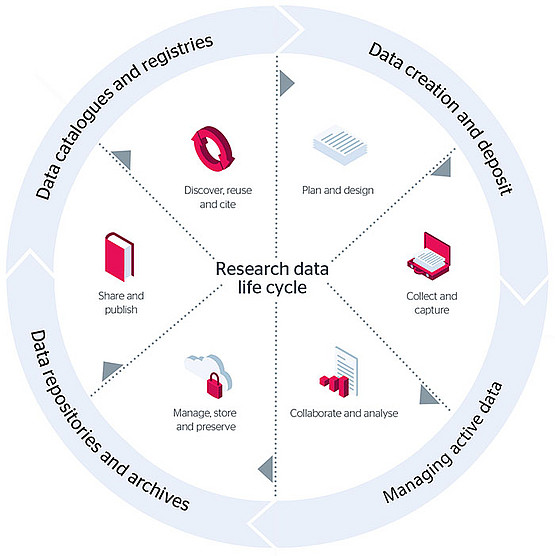
\includegraphics[width=.5\textwidth]{rdm-lifecycle-jisc.png}
	\caption[The life cycle of digital research objects]{The life cycle of digital research objects. License: JISC Research data management toolkit (\href{https://www.jisc.ac.uk/guides/rdm-toolkit}{www.jisc.ac.uk/guides/rdm-toolkit}), CC-BY-ND}
	\label{fig:rdm-lifecycle}
\end{figure}


\subsection{The FAIR guiding principles for scientific data management and stewardship}

Since their publication, the so-called \glsunset{FAIR}\gls{FAIR} principles \citep{wilkinson2016fair} have become guidelines for \gls{rdm} efforts for digital research objects.
They describe four measurable properties of research data that -- the better they are fulfilled -- serve the ultimate goal to improve the discoverability and reusability of data by machines and humans alike \citep{wilkinson2016fair}.
The \gls{FAIR}ness of data can be improved on each of the four related but separable major characteristics that are behind the \gls{FAIR} acronym (taken verbatim from \citet{wilkinson2016fair}):

\begin{itemize}
	\item \textbf{F}indable: To be Findable, (meta)data  are assigned a globally unique and persistent identifier (F1); data are described with rich metadata (F2); metadata clearly and explicitly include the identifier of the data it describes (F3);  (meta)data are registered or indexed in a searchable resource (F4)
	\item \textbf{A}ccessible: To be Accessible, (meta)data are retrievable by their identifier using a standardized communications protocol (A1); the protocol is open, free, and universally implementable (A1.1); the protocol allows for an authentication and authorization procedure, where necessary (A1.2);  metadata are accessible, even when the data are no longer available (A2)
	\item \textbf{I}nteroperable:  To be Interoperable, (meta)data use a formal, accessible, shared, and broadly applicable language for knowledge representation (I1); (meta)data use vocabularies that follow FAIR principles (I2); (meta)data include qualified references to other (meta)data (I3); and
	\item \textbf{R}eusable: To be Reusable, meta(data) are richly described with a plurality of accurate and relevant attributes (R1); (meta)data are released with a clear and accessible data usage license (R1.1); (meta)data are associated with detailed provenance (R1.2); (meta)data meet domain-relevant community standards (R1.3)
\end{itemize}

A pivotal factor for the importance of the FAIR principles is the increasing digitization of research practice, and with it, a rapid growth in research data \citep{dfg}.
Innovation relies on the ability to integrate new and existing data, and where the amount of data to discover, understand, and consolidate requires automation, research objects themselves need to become self-descriptive.
For this, the term ``machine-actionable'' is central to the \gls{FAIR} principles.
It is used to describe an ideal state in which a digital object provides detailed information (metadata) to an autonomously-acting, computational data explorer in two possible contexts: For one, as metadata about the object (``What is it?''), and second, as metadata about its content (``How do I process it?'') \citep{wilkinson2016fair}.
\todo{Add how the FAIR principles have become an internationally accepted standard - NFDI?}
\todo{add economic and scientific practice considerations for the FAIR principles}
Importantly, the \gls{FAIR} principles do not suggest specific metadata standards, implementations, or technology choices.
The following sections will outline \gls{rdm} requirements and solutions in the field of neuroimaging that work towards this goal.

%  The outcomes from good data management and stewardship, therefore, are high quality digital publications that facilitate and simplify this ongoing process of discovery, evaluation, and reuse in downstream studies.


% Internationally accepted standard
%The largest funding institution for the sciences and humanities and research in Germany, the \gls{grf}, states that access to data and software according the the FAIR principles are of comparable importance to science as access to publications \citep{dfg}




%Thus, the reusability of a research output is arguably its most important feature because of economical or efficiency considerations, as reusable research will speed up progress and curb costs.
%Reusing digital research outputs refers to the further use or utilization of any such research outputs inside or outside its original research context, by the original author or different actors.



\subsection{Research data management in neuroimaging}
\label{chap:k1-rdm-2}

%\[
%\left[
%\begin{tabular}{@{\quad}m{.3\textwidth}@{\qquad}m{.6\textwidth}@{\quad}}
%	\includegraphics[width=.7\linewidth]{qr_pub_niso.png} &
%	\raggedright%
%	\textbf{Related publications} \par
%	The following section contains a subset of the work presented in our original publication \citet{NISO2022119623}.
	%
%\end{tabular}
%\right]
%\]


Neuroimaging data poses a number of additional challenges for research data management.
For one, the field is characterized by complex datasets.
They typically encompass different modalities (such as imaging, electro-physiological, and behavioral measurements) and often entail several recording sessions.
The \gls{BIDS} \citep{gorgolewski2016brain} is a community standard for organizing and describing neuroimaging data, and is widely considered as a successful solution for data standardization in such datasets.
It defines common and modality specific schemes for file names and file organization, file formats, and metadata to accompany raw or derived data.
\gls{BIDS} has widespread and growing support for different neuroimaging modalities, and is made a common prerequisite by neuroscientific data portals such as OpenNeuro \citep{markiewicz2021openneuro} or processing tools such as BIDSApps \citep{gorgolewski2017bids}.
An example of an \gls{meg} dataset, structured to \gls{BIDS} or organized idiosyncratically, is shown in \cref{fig:BIDS}. \\
The storage demands of neuroimaging data are not trivial, either.
\gls{BIDS} regulates which file formats must be used for which data type, and focuses on open file formats for accessibility and compression to reduce disk space requirements.
But neuroimaging data are nevertheless sizable \citep{van2014human}.
And a growing awareness that robust findings require sufficiently long recordings \citep{li2021moving} as well as large and representative samples \citep{button2013power} \citep{turner2018small} leads to large-scale datasets such as the Human Connectome Project \citep{van2013wu}, the Adolescent Brain Cognitive Development Study (ABCD) \citep{casey2018adolescent}, or the UK Biobank (UKB) project \citep{matthews2015uk} that pose infrastructural challenges for storage, analysis, transfer and archival.
Moreover, in human neuroimaging, data underlies strict data protection regulations such as the \gls{HIPAA} in the United States or the \gls{GDPR} in Europe.
This requires compliance to variable terms of data usage agreements, and often involves idiosyncratic processes to retrieve data \citep{waitedata}.

% provenance
\begin{figure}
	\centering
	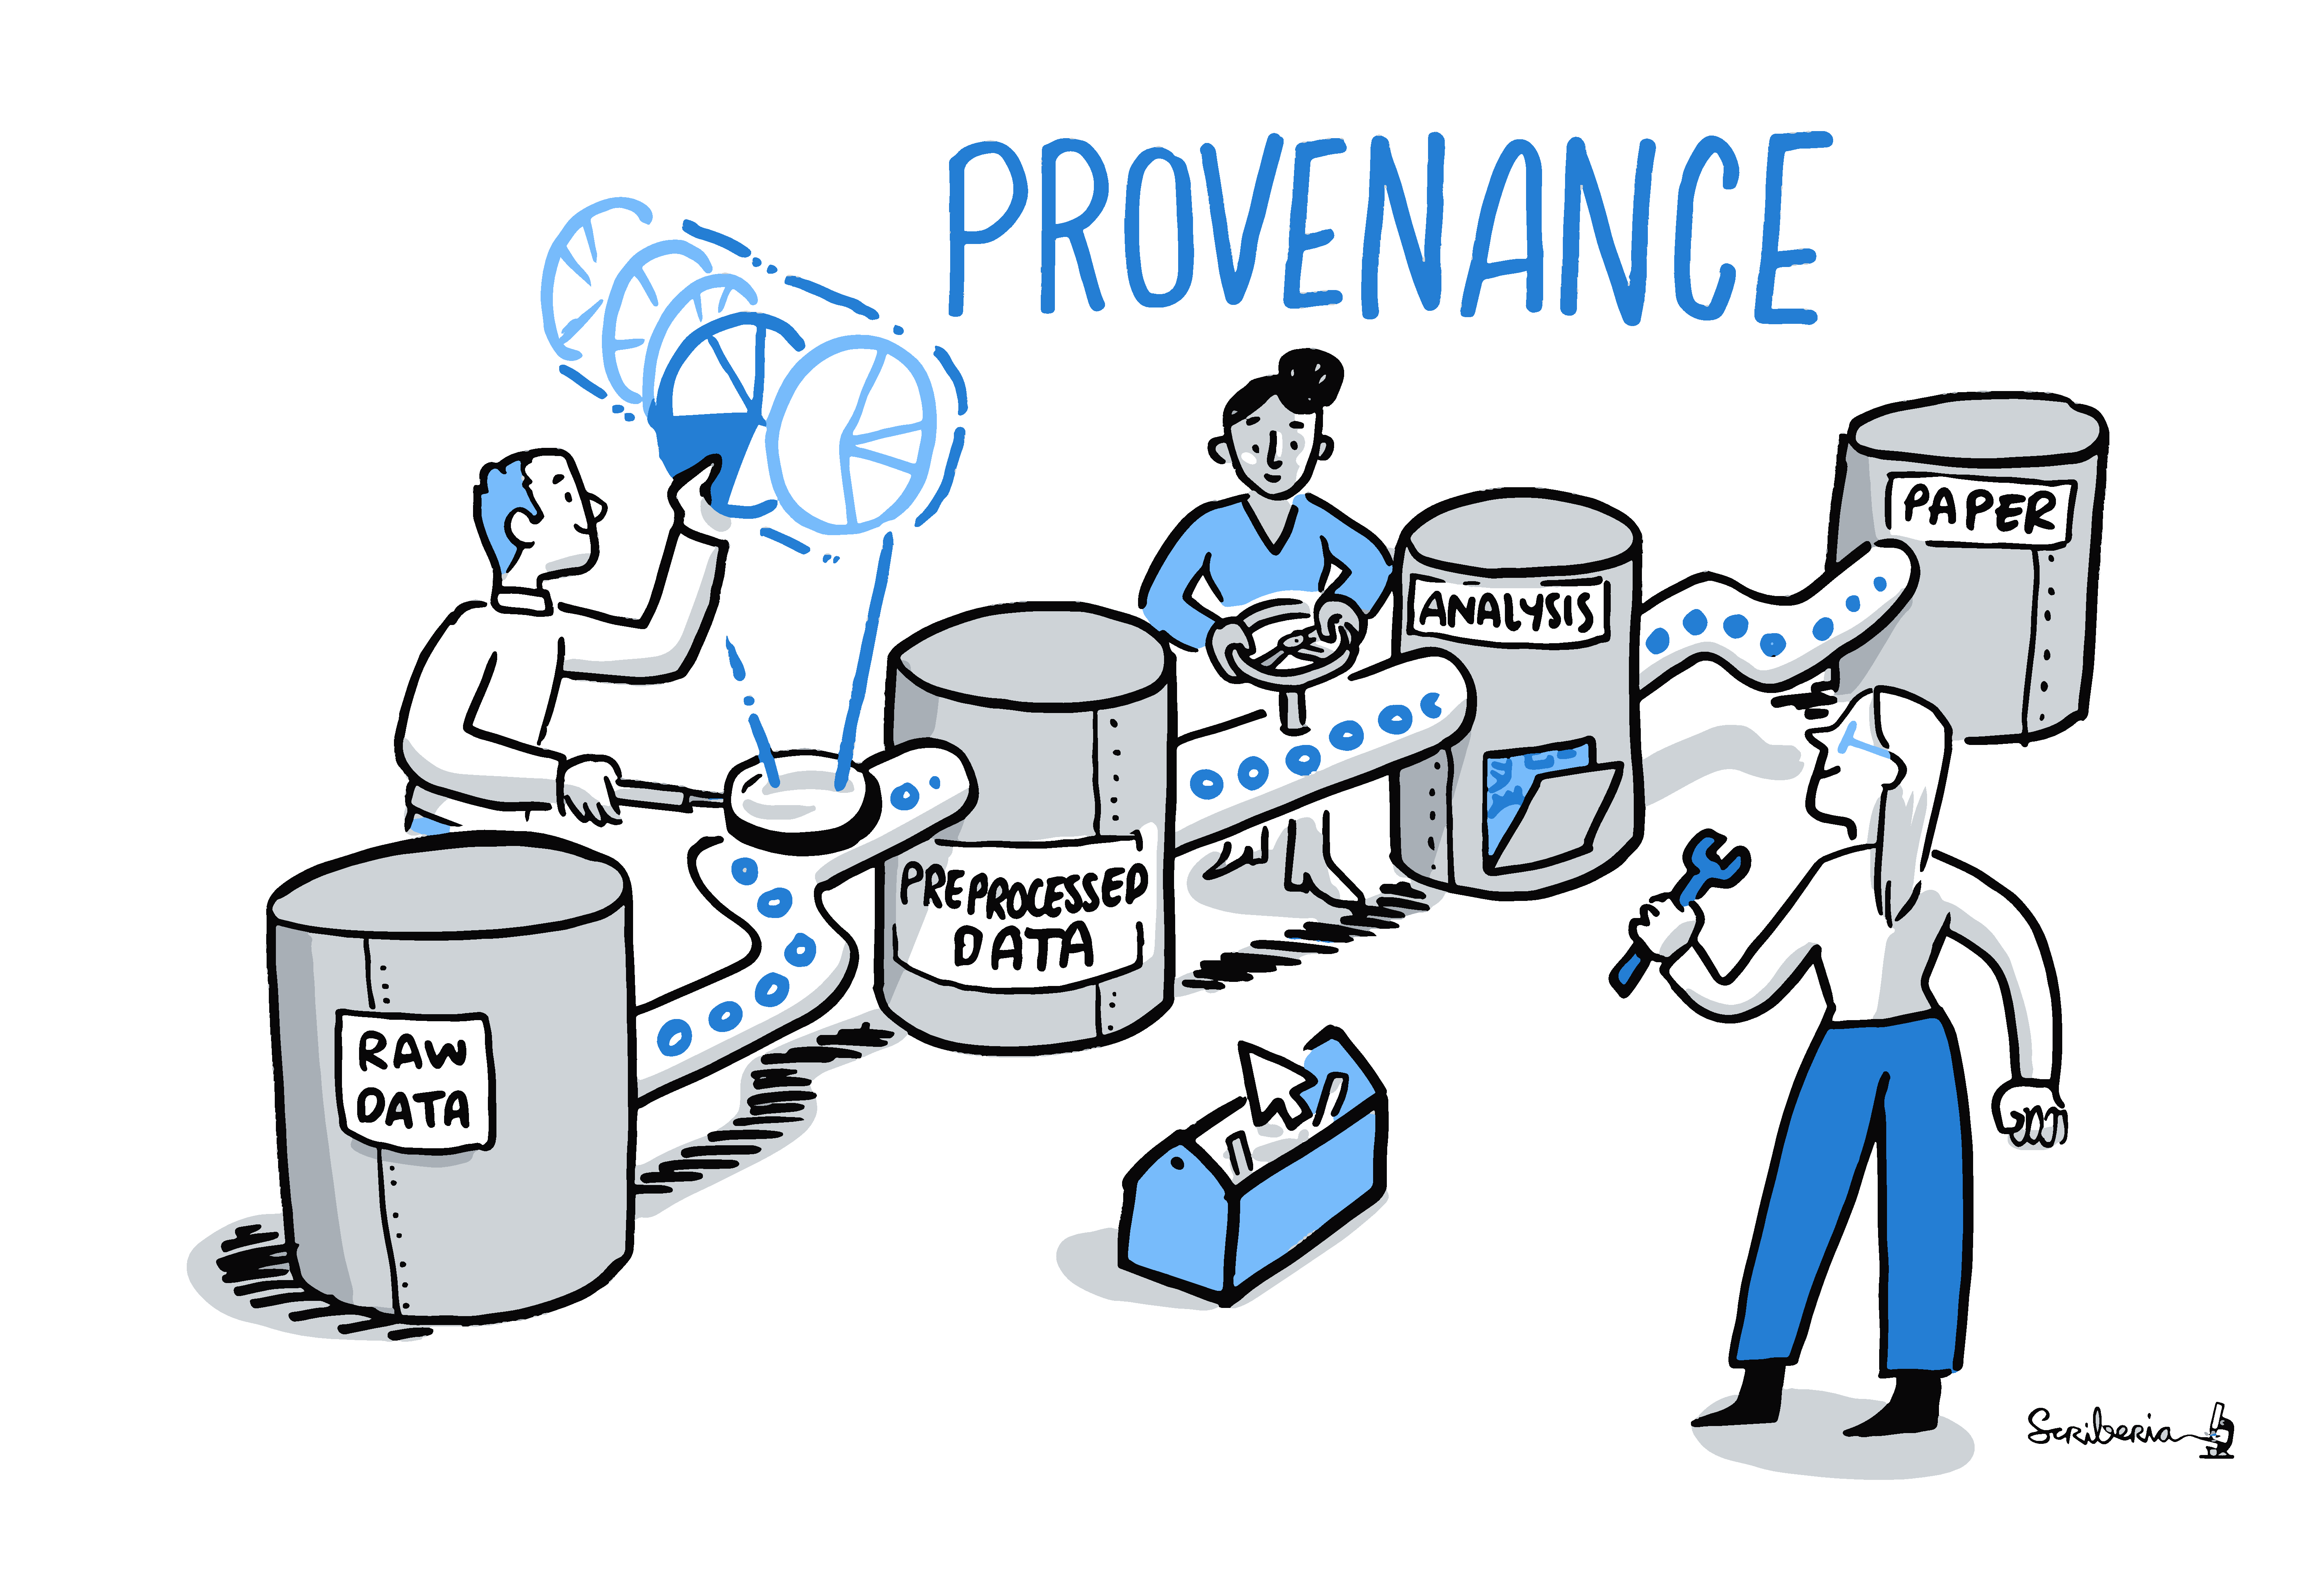
\includegraphics[width=.5\textwidth]{provenance.pdf}
	\caption[Provenance throughout the research process]{In multi-stepped analyses, a variety of choices affect the final outcome. Digital provenance, information about how tools, data, and actors were involved in the generation of file, is required to retrace, understand, and trust the decisions that led to a research outcome. Such provenance can be an outcome of good research data management. License: Scriberia and the Turing Way Project, CC-BY}
	\label{fig:prov1}
\end{figure}

\begin{figure}
{\scriptsize
  \begin{minipage}{.49\textwidth}
	\begin{forest}
		pic dir tree,
		for tree={% kleiner Zeilenabstand
		s sep=0.02cm}
		[memento/
		[memento\_001/
%		[Move\_correc\_SSS\_alignedinitial\_nonfitiso/
%		[1\_memento\_001\_ml83-1\_mc\_transforminitial.fif, file]
%		[2\_memento\_001\_ml83-1\_mc\_transforminitial.fif, file]
%		[3\_memento\_001\_ml83-2\_mc\_transforminitial.fif, file]
%		[data\_fix1.mat, file]
%		[data\_fix\_ft1.mat, file]
%		[data\_fix\_new1.mat, file]
%		[data\_fix\_reduced1.mat, file]
%		[delay\_photodiode\_subject\_long\_default\_realign\_only\_ICA1.mat, file]
%		[memento\_results\_ICA\_newall\_alignedinitial228.mat, file]
%		[memento\_results\_ICA\_newall\_alignedinitial461.mat, file]
%		[memento\_results\_ICA\_newall\_alignedinitial511.mat, file]
%		[num\_trials\_old\_ICA.mat, file]
%		[resultfile\_probs-1.mat, file]
%		[trial\_out\_ind.mat, file]
%		]
		[Move\_correc\_SSS\_realigneddefault\_nonfittoiso/
	    [1\_memento\_001\_ml83\_mc\_realigneddefault.fif, file]
	    [2\_memento\_001\_ml83-1\_mc\_realigned\_default.fif, file]
	    [3\_memento\_001\_ml83-1\_mc\_realigned\_default.fif, file]
	    [memento\_results\_ICA228.mat, file]
	    [memento\_results\_ICA455.mat, file]
	    [memento\_results\_ICA461.mat, file]
	    [memento\_results\_ICA511.mat, file]
	    [memento\_results\_ICA\_newall228.mat, file]
	    [memento\_results\_ICA\_newall455.mat, file]
	    [memento\_results\_ICA\_newall461.mat, file]
	    [memento\_results\_ICA\_newall511.mat, file]
	    [mri\_aligned.mat, file]
	    [num\_trials\_old\_ICA.mat, file]
	    [outfile\_new\_all.mat, file]
	    [resultfile\_new\_all.mat, file]
	    [template\_grid.mat, file]
	    [trial\_out\_ind.mat, file]
		]
		[Raw/
		[1\_memento\_001\_ml83.fif, file]
		[2\_memento\_001\_ml83-1.fif, file]
		[memento\_001\_ml83-2.fif, file]
		]
		]
		]
	\end{forest}
\end{minipage}
\quad
  \begin{minipage}{.49\textwidth}
	\begin{forest}
		pic dir tree,
		for tree={% kleiner Zeilenabstand
			s sep=0.02cm}
		[memento/
		[dataset\_description.json, file]
		[participants.json, file]
		[participants.tsv, file]
		[README, file]
		[sub-001/
		[meg/
		[sub-001\_acq-calibration\_meg.dat, file]
		[sub-001\_acq-crosstalk\_meg.fif, file]
		[sub-001\_coordsystem.json, file]
		[sub-001\_task-memento\_channels.tsv, file]
		[sub-001\_task-memento\_events.tsv, file]
		[sub-001\_task-memento\_log.tsv, file]
		[sub-001\_task-memento\_meg.json, file]
		[sub-001\_task-memento\_split-01\_meg.fif, file]
		[sub-001\_task-memento\_split-02\_meg.fif, file]
		[sub-001\_task-memento\_split-03\_meg.fif, file]
		]
		[sub-001\_scans.tsv, file]
		]
		]
	\end{forest}
\end{minipage}
}
\caption[An example of BIDS]{A real-world example of a single subject's MEG acquisition. The left side shows the file tree of the data from a project directory with an idiosyncratic. It includes a mix of raw data, preprocessed data, and intermediate results, and the naming scheme is inconsistent. The right side shows the same subject's data, but structured according to \gls{BIDS}. The naming scheme is consistent, and apart from raw MEG data the directory includes metadata files from the experiment and acquisition machine that are required to understand the data.}
\label{fig:BIDS}
\end{figure}

Processing of neuroimaging data usually involves multi-stepped workflows from acquisition through analysis to archival, and those frequently require several different software tools at every step \citep{poline2011}\citep{NISO2022119623}.
The amount of possible combinations of methods, parameters, and tools in neuroimaging analyses is thus large \citep{bowring2019exploring}.
But variations in analytic choices affect numeric results and conclusions \citep{silberzahn2018}.
In the field of task-based fMRI, \citet{botvinik2020variability} found highly variable conclusions when they instructed 70 independent research teams to analyze the same dataset with tools and methods of their choice to test the same hypotheses.
A similar project, EEGManyPipelines, is currently ongoing in the field of EEG (\href{https://eegmanypipelines.org/}{eegmanypipelines.org}).
One central aspect \gls{rdm} thus needs to provide in neuroimaging is precise information about how tools, data, and actors were involved in the generation of a file.
This \textit{digital provenance}  (illustrated \cref{fig:prov1}) is not meant to decrease the analytical variability.
Instead, it captures thorough, machine-actionable processing descriptions that are necessary to investigate differences between analysis outcomes, reproduce, or reuse them.
Despite reporting guidelines for MRI \citep{nichols2017best}, MEG \citep{pernet2020issues}, and EEG \citep{styles2021towards} studies, traditional publications still regularly fail to report all relevant details about recording, processing, and analysis (see e.g., \citet{vsovskic2022better}).

\todo{add more RDM peculiarities of neuroimaging here. Maybe deep dive into computational modelling}

Careful \gls{rdm} is necessary to translate complex data efficiently into scientific insights.
Given these specific complexities in neuroimaging, solutions to these challenges often arise from the community of researchers.
The following section will highlight one of several software tools that aids with the complex task of research data management: DataLad \citep{Halchenko2021}.
A subsequent chapter, \cref{chap:k2}, will later focus on how research data management is a prerequisite of reproducible research, specifically with regards to software environments and large sample sizes.
In addition, \cref{chap:k2} will highlight pragmatic approaches to \gls{rdm} that can be embedded in standard research practice and contribute to the FAIRification of data, even in absence of established metadata formats.



% link to chapter 3: Research data management is a prerequisite of reproducible research

\section{DataLad as a software solution for research data management challenges}

\[
\left[
\begin{tabular}{@{\quad}m{.3\textwidth}@{\qquad}m{.6\textwidth}@{\quad}}
	\includegraphics[width=.7\linewidth]{qr_pub_datalad.png} &
	\raggedright%
	\textbf{Related publications} \par
	The following section provides an overview of the features of the software tool DataLad and their use for research data management.
	The reader is invited to refer to our original publication \citep{Halchenko2021} for a more detailed description.%
\end{tabular}
\right]
\]

%This introduces DataLad as a software solution for research data management

\subsection{An overview of features and their use for \gls{rdm}}

Although many solutions to common challenges exist, putting \gls{rdm} into practice remains a complicated endeavor:
In most neuroimaging studies, scientific insights are created from well-described raw data and its derivatives.
Standards and repositories as mentioned in \cref{chap:k1-rdm-2} form a basis for managing, storing and sharing them, and being able to efficiently retrieve and update these research objects across a variety of available storage options is an important part of \gls{rdm} \citep{borghi2018data}.
However, homogeneous data transport is complicated by disconnected and non-interoperable hosting solutions.
Different storage services can require different protocols, means of authentication, or other idiosyncrasies (CITATION NEEDED). \\
Over the course of a research project, often as part of the standard, multi-stepped processing workflow \citep{poline2011}, data also evolve and change:
Continued acquisitions enlarge the raw dataset.
Transformations to community standards such as \gls{BIDS} \citep{gorgolewski2016brain} change file formats, dataset organization, or enrich available metadata.
Continuous quality control processes or accidental findings can bring errors to light and improve datasets with fixes (e.g., CITATION NEEDED).
In the case that data or other research objects were subject to change over the course of a project, there is a need to identify which exact version has been used -- otherwise, the reproducibility of a result is threatened (CITATION NEEDED). \\
Likewise, projects might draw insights from only a subset of a dataset, such as only specific modalities, tasks, or participants, despite much greater data availability.
If the original dataset, however, is only available as a bulk download, a project has heavier disk space demands on storage solutions than their eventual data requirements.
Especially in the age of big data neuroscience \citep{bzdok2017inference}, downloads or storage of standard large-scale datasets can become infeasible \citep{horien2021hitchhiker} \citep{grisham2016proposed}. \\
Finally, \textit{digital provenance}, the information bout how tools, data, and actors were involved in the generation of a digital research outcome is crucial to understand and reproduce a result, but rarely fully transparent and documented, let alone machine-readable or actionable.
% NISO The ability to manage data and metadata and track the data-analysis process provides a basis for rigor and reproducibility.


DataLad (\href{http://datalad.org}{datalad.org}) \citep{Halchenko2021} is a Python-based, MIT-licensed software tool for the joint management of code, data, and their relationship, developed with the aim to assist with common \gls{rdm} tasks in science.
Its main features provide solutions to the difficulties outlined above:
Building up on established open source version control tools, Git (CITATION) and git-annex (CITATION NEEDED), DataLad provides the ability to version control data of any size or type.
Bridging a large variety of storage and Git repository hosting services with its interoperability layer, it streamlines procedures to consume, publish, and update digital data, and unifies authentication procedures for an end user.
Due to a separation between file content and file identity metadata, DataLad allows
- fine grained access control for data providers
- downloads at single file granularity for data users
- lightweight but actionable access to data

With dedicated functionality to capture complete and actionable process provenance of data transformations and allow automatic re-computation, DataLad can record machine-actionable metadata how files came into existence.
Based on Git's submodule mechanism, DataLad allows for modular structuring of ...
 for  and to link them as precisely versioned, lightweight
dependencies. DataLad helps to make science more reproducible and FAIR (Wilkinson et al.,
2016). It can capture complete and actionable process provenance of data transformations to
enable automatic re-computation.

Fundamental to DataLad's functionality is the concept of the ``DataLad dataset'', DataLad's central data structure.
On a technical level, it is a joint Git/git-annex repository.

%VAMP
 version control. If used appropriately, version control tools associate a unique identifier and basic provenance with each revision, and thus enable the identification of precise version states of digital files or collections of files. With other useful features such as built-in collaboration and the ability to save and revert changes, it also facilitates common scientific workflows, and has been increasingly adopted for research data management (RDM) in science \citep{nord2019towards} \citep{strupler2017reproducibility} \citep{bryan2018excuse} \citep{corti2019managing}.

%% from datalad paper:


Code, data and computing environments are core components of scientific projects. While
the collaborative development and use of research software and code is streamlined with es-
tablished procedures and infrastructures, such as software distributions, distributed version
control systems, and social coding portals like GitHub, other components of scientific projects
are not as transparently managed or accessible. Data consumption is complicated by discon-
nected data portals that require a large variety of different data access and authentication
methods. Compared with code in software development, data tend not to be as precisely
identified because data versioning is rarely or only coarsely practiced. Scientific computation
is not reproducible enough, because data provenance, the information of how a digital file
came to be, is often incomplete and rarely automatically captured. Last but not least, in
the absence of standardized data packages, there is no uniform way to declare actionable
data dependencies and derivative relationships between inputs and outputs of a computa-
tion. DataLad aims to solve these issues by providing streamlined, transparent management
of code, data, computing environments, and their relationship. It provides targeted interfaces
and interoperability adapters to established scientific and commercial tools and services to
set up unobstructed, unified access to all elements of scientific projects. This unique set of
features enables workflows that are particularly suited for reproducible science, such as ac-
tionable process provenance capture for arbitrary command execution that affords automatic
re-execution. To this end, it builds on and extends two established tools for version control
and transport logistics, Git and git-annex.


\subsection{Software adoption and relevance}

DataLad does not employ tracking code.
As such, the exact number of its users is not known.
However, download statistics from the major Python package managers \texttt{pip} and \texttt{conda}, and popularity statistics from users of the Debian operating system can provide rough references.
According to pypistats.org, the main DataLad Python package was downloaded from the Python Package Index 300 times per day on average in May 2023.
The Python distribution Anaconda (anaconda.org) counts a total of 333932 downloads of the software throughout versions 0.9.3 (April 2018) and 0.18.3 (May 2023), averaging 180 downloads per day.
The \texttt{popularity-contest} software is a Debian package that, if installed on a users system, reports anonymous statistics about most-used Debian packages.
This data is aggregated into a popularity contest.
According to it, in May 2023 between 0.04 and 0.05 percent of systems reporting statistics have an installation of the DataLad Debian package, or the equivalent python3-datalad Debian package.
All of these sources contain biases that limit conclusion to the number of users, though.
Installations via Python package managers are commonly performed by individual end users, whereas installations of Debian packages can correspond to system-wide installations on multi-user systems such as high performance computing infrastructure.
Likewise, upgrades of existing installations to more recent versions are included in these data, as well as temporary installations of the software in automated continuous integration test suites.
Nevertheless, download statistics confirm that it is an actively used tool with a user base that exceeds the circle of its developers by far.
This is also confirmed by citations of the academic paper, totaling 51 1.5 years after its publication by \citet{Halchenko2021}, and active contributor community around the source repository on GitHub, currently amounting to 48 individuals with committed code contributions.



\pagebreak

